\documentclass[conference]{IEEEtran}
%\documentclass[onecolumn, draft]{IEEEtran}
\IEEEoverridecommandlockouts
% The preceding line is only needed to identify funding in the first footnote. If that is unneeded, please comment it out.
\usepackage{cite}
\usepackage{amsmath,amssymb,amsfonts}
\usepackage{algorithmic}
\usepackage{graphicx}
\usepackage{textcomp}
\usepackage{xcolor}
\usepackage{tikz,pgfplots}
\def\BibTeX{{\rm B\kern-.05em{\sc i\kern-.025em b}\kern-.08em
    T\kern-.1667em\lower.7ex\hbox{E}\kern-.125emX}}
\begin{document}

\title{Slice-and-cluster: Summarization of discrete event signals patterns with event clustering on time segments
%\thanks{Identify applicable funding agency here. If none, delete this.}
}
\author{\IEEEauthorblockN{1\textsuperscript{st} Anonymous}
\IEEEauthorblockA{\textit{Anonymous } \\
}
\and
\IEEEauthorblockN{2\textsuperscript{nd} Anonymous}
\IEEEauthorblockA{\textit{Anonymous} \\
}
}

%\author{\IEEEauthorblockN{1\textsuperscript{st} Vanessa Cedeno-Mieles}
%\IEEEauthorblockA{\textit{Network Dynamics and Simulation Science Laboratory, } \\
%\textit{Biocomplexity Institute (of Virginia Tech)}\\
%Blacksburg, VA, USA \\
%\textit{Escuela Superior Politecnica del Litoral, ESPOL} \\
%Guayaquil, Ecuadort \\
%vcedeno@vt.edu}
%\and
%\IEEEauthorblockN{2\textsuperscript{nd} Sandeep Gupta}
%\IEEEauthorblockA{\textit{Network Dynamics and Simulation Science Laboratory, } \\
%\textit{Biocomplexity Institute (of Virginia Tech)}\\
%Blacksburg, VA, USA \\
%sandeep@vt.edu}
%}

\maketitle

\begin{abstract}
We present an approach for summarizing a given set of discrete valued time series. Our work is generalization of~\cite{Kiernan:constructing} which presents a formulation and an optimal strategy to summarize binary valued time series. 
  Summarization, concisely represents a large event sequence emphasizing the fundamental characteristics of the entire data set. Having a global overview of the dataset allows the user to explore different options of where to start a more detailed analysis. Our approach yields summaries that  1)  are concise and accurate, outputting a short and correct description of the input data. 2) provide a global data model, i.e., describe the global structure and how it evolved through the time dimension. 3) provide a local pattern model, describing local patterns so the user can identify similar behavior between events during a segment in time. and 4) is parameter-free, which means that apart from the initial event sequence, additional information need not be provided by the user.
  We use the Minimum Description Length (MDL) principle to detect regularities and compress data. We apply two dynamic programming algorithms to optimally and automatically segment the sequences in time and cluster events to discover similarities in polynomial time. Experiments on synthetic datasets effectively and efficiently summarize event sequences, finding correct cuts and clusters. Experiments on real datasets, including Ebola cases in Liberia, and the Global Landslide Catalog, demonstrate that our summarization finds useful patterns and tell stories validated with the analysis made by experts in the respective dataset domain.
\end{abstract}

\begin{IEEEkeywords}
summarization, discrete event signals, minimum description length, dynamic programming, clustering
\end{IEEEkeywords}


\section{Introduction}

\begin{figure}[!tbh]  %[htbp]
%\vspace*{-0.1in}
  \begin{center}
       \includegraphics[trim = 0.5in 0in 0in 0in, clip,scale=0.35]{images/intro.pdf}
  \end{center}
%  \vspace{-0.2in}
   \caption{The raw data in the top figure shows a timeline by day, from 1 to 160. Each dot in the raw data, represents a daily event frequency from 150 events. These events follow group patterns identified by the Slice-and-cluster summarization in the bottom figure. The output of the summarization is, first, the segmentation of the time dimension \{1-15, 16-25, 26-45, 46-70, 71-80, 81-160\} and second, the local clusters for each of these time segments. Each local cluster is a list of events id's that form part of the cluster and the summarization is a daily rate. Because this is synthetic data we know the list of events that conforms a pattern, and the algorithm accurately detects them. For visual aid the local clusters are represented by a color box of the pattern an event belongs to, if the events are all from different patterns but can be represented by the same daily rate the color boxes are combined.
}
  \label{fig:intro}
\end{figure}

Complex dynamical systems, from computer systems, epidemics, to natural events, are only observable through the temporal events they emit.  Quite often, actions and policies, requires an understanding of the targeted complex system. Usually, this includes, detecting changes in the frequency of event occurrences as a function of time and finding explanations for the changes.  A sequence of these events consists  of pairs $(e,t)$, where $e$ is the type of event and $t$ is the occurrence time. Large amount of sequences of events log are being collected from different environments, like sensors, disaster management, epidemic control, etc. Iterating through different event pattern mining techniques to discover hidden temporal patterns from these logs can take time. Also, these techniques outputs involve a large number of recurring patterns infeasible for manual analysis. Before committing to a detailed analysis and the depuration of it's potentially massive results, is clever to have an overview of the entire data log. Event summarization is a process that summarizes the characteristics of the events within a system logs. In other words, event summarization emphasizes the fundamental characteristics of an entire data set. Our main objective is to provide an overview of multivariate event sequences in a glimpse. Because of this, our summarization will 1) be concise and accurate, outputting a short and correct description of the input data. 2) Provide a Global data model, describing the global structure and how it evolved through the time dimension. 3) Provide a Local pattern model, describing local patterns so the user can identify similar behavior between events during a segment in time. And 4) parameter free, which means than apart from the initial event sequence, additional information should not be provided by the user. Figure \ref{fig:intro} shows an illustrative example. 




Many of the recent work in event summarization can be divided between two methodologies, frequency change \cite{Kiernan:constructing,wang:algo} and temporal dynamics \cite{jiang:natural,Peng:2007,Schneider:2010,Tatti:2012}.
%% TODO: might be good give an example right here and introduce time segmentation and groups. introduce it not for event sequence but general time series. 
%% 
%% TOOD: Is kiernan's frequency change or temporal dynamics
%% TODO: explain frequency change
%% TODO: explain temporal dynamics
In \cite{Kiernan:constructing}, the summarization problem is described as an optimization problem. MDL is used to find a balance between the summary's length and description's accuracy. Two dynamic programming algorithms are used to solve the problem in polynomial time. In the end it provides an overall description of the event sequences, including local similarities of the events for each segment. 

%% TODO: first describe the goal/problem solved the paper and then the approach
In \cite{wang:algo} the previous algorithm was extended by adding inter-segment information to describe the event generation process. Like in \cite{Kiernan:constructing} the summarization problem is formulated as an optimization problem. It finds the best segmentation and a Hidden Markov Model (HMM) describes an event sequence with the minimum amount of information. The MDL principle is used to represent the event sequence. A HMM is used to model the state transition of a system. To solve the problem of disconnected segmentations in the summarization the HMM takes into account the correlation between the occurrence of events. A limitation of this approach is that the experiment on real data is limited, and it is not clear how high interpretability is achieved. 

%% TODO: needs more setup: what is same-type, what is different-type, what is inter-arrival. Would be good repeat the precise problem being addressed
In \cite{jiang:natural} an event sequence is summarized using inter-arrival histograms to capture the temporal relationship among events. The temporal relationships are among same-type and different-type events, then it finds a set of disjoint histograms to summarize the input event sequence based on MDL. At the end, the resulting summary is represented as an event relationship network. It uses MDL and multi-resolution analysis for pruning the problem space. An event sequence is decomposed into many disjoint subsets and periodic patterns and correlation patterns are used to describe each subset. The inter-arrival histograms show event patterns and capture temporal dynamics of events.
%% TODO: does this work perform time seqmentation



These approaches \cite{Kiernan:constructing,wang:algo,jiang:natural} describe a concrete event summarization method, similar to the one we are proposing. For the frequency change approach, a segmentation model is provided. Each segment is described by a local model where the event types are grouped and clustered by frequency similarity. The temporal dynamics approach intents to reveal how the sequence changes over time. This can be done through the temporal dynamics of the segments or the temporal dynamics among the events. These approaches also deal with unique counts of events, this means that multiple events of the same type occurring at point $t$, are ignored as duplicates and counted as one occurrence. There is not straightforward extension for a model describing binary values (bv) event sequences to be able to use discrete values (dv) event sequences instead. Our work generalizes \cite{Kiernan:constructing} approach for discrete-valued event sequences. This means other models like \cite{wang:algo,jiang:natural}  can use our generalization to apply their own summarization methods. 

Other summarizations define their own methods for summarizing event sequences. In \cite{Peng:2007} a divide-and-conquer process is employed to extract temporal patterns based on entropy ranking and an Event Relationship Network (ERN) is constructed to provide concise representations. In \cite{Schneider:2010} temporal properties are mined from logged events maintaining these invariants during summarization. It uses coarsening to explore the representations space starting with smaller representations. In \cite{Aharon:2009} a sequential text clustering algorithm automatically discovers, the templates generating the messages, in system event logs. Then a second algorithm discovers patterns of messages that represent processes occurring in the system. In \cite{Tatti:2012} MDL is used to identify the set of sequential patterns that summarizes the data best. It formalizes how to encode sequential data using sets of serial episodes,
and uses the encoded length as a quality score. One algorithm selects a good pattern set from a large candidate set, while a second algorithm is parameter free and mines pattern sets directly from the data. 

After reviewing these methods we can see how there is no problem that can be tackle by one algorithm or model. There is no optimal summarization for real world data. Also, there is no generalization for any method describing binary values event sequences to be extended to discrete values event sequences. This is why we propose an algorithm that produces an optimal high level representation of the event sequences generalizing the generative model used for bv event sequences for dv event sequences.


\subsection{Our approach}
\begin{itemize}
\item We present a parameter-free optimal summarization in polynomial time using MDL and Dynamic Programming.
\item Our model identifies similarities between event sequences through time. Segmentation provides a high level overview describing the global structure and how it evolved through the time dimension and each of these segments will be clustered to discover local similarities between the series.
\item To test the effectiveness and efficiency of our model, we design two sets of experiments on both synthetic and real datasets. By generating an artificial dataset we are capable of identifying the optimal summarization and in this way test the accuracy and limitations of our model. The summarization of a real world dataset is validated with analysis made by experts in the respective dataset domain.
\end{itemize}
\subsection{Contributions}
In summary, our contributions are: 
\begin{itemize}
\item A novel, parameter-free, summarization-based approach to analyze event sequence data and create optimal global summaries using Minimum Description Length and Dynamic Programming. 
\item We generalize the generative model used for binary valued event sequences for discrete valued event sequences.
\item We validated our algorithms through a synthetic dataset generator. The generated datasets have known segments and clusters. The validation step entail checking if our proposed algorithm can pick the segments and cuts in presence of, varying magnitude, of  noise
  
\item  We present summarization results  on  real datasets which have been analyzed and reasoned upon by experts from that domain. We show that summarization produced by our algorithm corroborates with that of domain expert's analysis.

 

\end{itemize}
The rest of this paper is organized as follows. Section 2 introduces the notation and defines the problem. Section 3 discusses background theory. Section 4 describes our approach for the model. Section 5 describes the optimal solution for the model and it's time complexity. Section 6 contains experiments with artificial and real datasets. Section 7 discusses related work. Section 8 presents conclusions and future work.







\section{Notation and Problem Statement}
\subsection{Notation}
Table \ref{tab:notation} summarizes the major notations used in this and subsequent sections. 
\begin{table}[!h]
\centering
    \caption{Notation}     
    \label{tab:notation}
    \begin{small}
    \begin{tabular}{|ll|l}
    \hline
    {\bfseries Symbol} & {\bfseries  Description}      \\
    \hline
    $n$ & length of timeline  \\    \hline
    $m$ & number of event types \\    \hline
    $\epsilon=\{E_1,E_2,...,E_m\}$ & set $\epsilon$ of event types\\  \hline
    $S$ & event sequence, $m \text{ x } n$ array \\    \hline
    $S (i, t) = x$ & event $E_i$ has x occurrences at time $t$\\    \hline
    $S = \{S_1,\dots ,S_k\}$ & summarized S with k segments \\    \hline
    %$M = \{M_1,\dots ,M_k\}$ & local model for each of the k segments \\    \hline
    $M_i = \{X_{i1},\dots ,X_{i\ell}\}$&groups of events in local model $M_i$\\    \hline
    $I$ & interval $I \subseteq [1,n]$ \\    \hline
    $S_i=S[I]$ & segment defined over interval $I$ \\    \hline
    $n(E_j,I)$ & occurrences of $E_j$ at interval $I$ \\   \hline
    $X_{ij}$& group in $M_i$ from segment $S_i$ \\   \hline
    $\lambda(X_{ij})$ &average number of any event  \\  
    &occurrence in group $X_{ij}$\\  \hline
    $\lambda_{d}(X_{ij})$ &daily average number of any event \\  
    &occurrence in group $X_{ij}$ \\    \hline
    $LGM$ & Code length for the global model  \\    \hline
    $LLM$ & Code length for the local model  \\    \hline
    \end{tabular}
    \end{small} 
\end{table}

We have a set $\epsilon$ of $m$ event types, $\epsilon=\{E_1,E_2,...,E_m\}$. A pair $(E,t)$, describes that the event $E$ occurs at time $t$. We have discrete timelines in the interval $[1,n]$, in which the occurrence times of events are positive integers. An event sequence can be denoted as $S$ and records the event occurrences during the time range $[1,n]$. $S$ can be denoted as an $m\text{ }x\text{ }n$ matrix, where $S(i,t)=x$ denotes that the event $E_i$ has a number of $x$ occurrences at time $t$. Given interval $I \subseteq [1,n]$, $S[I]$ is a segment defined over the time interval $I$. $S_i=S[I]$ and denotes the $m\text{ }x\text{ }|I|$ projection of $S$ on the interval $I$. The sum of the occurrences of $E_j$ in interval $I$ is denoted as $n(E_j,I)$.


\subsection{Problem Statement}

Given an event sequence $S$ and records of occurrences for the events $E_i \in S$ in the timeline $[1,n]$, find integer $k$ and a segmental grouping $M$ of $S=\{S_i,\dots,S_k\}$ with the best local model grouping $M_i$ for each $S_i$.
We want our summarization to provide a global description that 1) shows how often do the events occur. 2) Shows how the frequency of occurrences change in the course of time. 3) Find related events that might provide an explanation for the changes in frequency.

We want our model to segment the timeline and cluster event sequences based on their frequency of occurrence. Figure 
\ref{fig:cuts} 
shows the actual segmental grouping that our model finds for this event sequence. The model cuts the timeline in three segments [1,8], [9,17] and [18,30]. In the first segment, two groups consist of event sequences $\{E_1,E_2\}$ and $\{E_3\}$, respectively. In the same way the second segment groups $\{E_1,E_3,E_2\}$ and the third segment groups$\{E_1\}$ and $\{E_3,E_2\}$.

\begin{figure}[h]
%\scalebox{0.93}{
\begin{tikzpicture}
 \begin{axis}[
 width=4.05in,
xmin=1,
xmax=31,
ymin=0,
ymax=0,
 y=0.1cm,
hide y axis,
axis x line*=bottom,
xtick={1,9,18,31},
]
\end{axis}
\end{tikzpicture}

\scalebox{0.389}{

    \begin{tabular}{|cccccccc|ccccccccc|ccccccccccccc|}
        \hline
0&1&1&0&1&0&4&1&16&17&6&9&11&8&12&9&11&2&1&2&0&2&1&0&0&1&1&0&2&0\\\cline{18-30}
1&1&0&0&0&2&1&0&11&15&11&9&9&3&8&13&6&12&27&17&26&26&18&30&21&20&28&22&23&17\\\cline{1-8}
14&15&8&13&8&14&14&13&16&10&13&4&5&14&6&12&17&23&30&25&22&17&35&28&20&28&28&35&23&23\\\hline
\multicolumn{20}{c}{}\\
\multicolumn{8}{c}{$\{E_1,E_2\}\{E_3\}$}&\multicolumn{9}{c}{$\{E_1,E_3,E_2\}$}&\multicolumn{13}{c}{$\{E_1\}\{E_3,E_2\}$}\\
    \end{tabular}
    }


 \caption{Visual representation of our event sequence summarization. Here n=30 and m=3. The model cuts the timeline in [1,8] grouping $\{E_1,E_2\}\{E_3\}$. Then cuts [9,17] grouping $\{E_1,E_3,E_2\}$. Finally it cuts [18,30] grouping $\{E_1\}\{E_3,E_2\}$.}
\label{fig:cuts}
\end{figure}

The summarization of the event sequences partition $S$ into $k$ segments, $S=(S_1, S_2,..., S_k)$ where $0 <k \leq n$. After segmentations there are $k+1$ cuts, $\{c_1, c_2, ..., c_i, ...,c_{k+1}\}$ to represent the boundaries of the $k$ segments. Here, $c_1=1$, $c_{k+1}=n+1$ and the rest of the boundaries $c_j$ take values between $2\leq j \leq k$. A model $Mi$ partition the rows of $S_i$, clustering the event types in $\epsilon$ into $\ell$ groups $\{X_{i1},...,X_{i\ell}\}$ such that $X_{ij} \subseteq \epsilon$, $X_{ij} \cap X_{ij'}=\emptyset$ for every $j \neq j'$ and $1\leq j, j' \leq \ell$. For each group $X_{ij}$ the parameter $\lambda(X_{ij})$ will be defined as the average number of any event part of group $X_{ij}$ within the data segment $S_i$. $\lambda_{daily}(X_{ij})$ will be defined as the daily average number of any event, part of group $X_{ij}$, within the data segment $S_i$. $S (i, t) = x$ shows that event $E_i$ has x occurrences at time $t$, where $x\geq 0$. In Figure \ref{fig:cuts}, if $E_1$ represents the first row, $E_2$ represents the second row, and $E_3$ represents the third row; S(1,7)=4 and S(2,7)=1. $n(E_j,I)$ represents the number of occurrences of $E_j$ at interval I. In Figure \ref{fig:cuts}, if $I=[1,8]$ then $n(E_1,I)=8$ and $n(E_2,I)=5$. Also, if $I=[1,8]$ is represented by a local model with the following group of events, $M_1=\{X_{11}, X_{12}\}$, with $X_{11}=\{E_1, E_2\}$ and $X_{12}=\{E_3\}$; then $\lambda_d(X_{11})=\frac{n(E_1,I)+n(E_2,I)}{I * |X_{11}|}=\frac{13}{8*2}=0.81$, and $\lambda_d(X_{12})=\frac{n(E_3,I)}{I * |X_{12}|}=\frac{99}{8*1}=12.38$.

\subsection{Challenges}
\begin{enumerate}
\item There is no generalization for any method describing binary values event sequences to be extended to discrete values event sequences.
\item The problem statement defines a compressing pattern problem; giving sequence $S$, there are multiple window conditions, and for each condition a set of candidate patterns $\mathcal{M}$ is presented. Finding an optimal model for this definition is NP-Hard \cite{Lam:2014}.
\item There is no optimal summarization for real world data.

\end{enumerate}

We provide solutions for these challenges in the subsequent sections, 1) Section \ref{sec:poisson}, 2) Section \ref{sec:time}, 3) Section \ref{sec:realdata}.



\section{Theory}
In this section we introduce the Minimum Description Length (MDL) principle.
\subsection{MDL}
The concept of MDL was defined by Rissanen \cite{rissanen:short, rissanen:mdl}. It has its roots in information theory and can be dated back to the concept of the Kolmogorov Complexity and the invariance theorem.
%, introduced and proved independently by \cite{Kolmogorov65, Chaitin69, Solomonoff64}. 

A formal language is needed to describe a data sequence. For example, a general purpose language. The Kolmogorov Complexity of a sequence, is the length of the shortest computer program that produces the initial sequence as an output. The complexity is the minimal description length. The lower the Kolmogorov complexity of a sequence the more regular it is. 
If there is a random sequence, the Kolmogorov complexity is close to the entropy.

\textbf{Entropy: } Entropy measures the uncertainty associated with a random variable. The entropy of a random variable $X$ denoted $H(X)$ is a lower bound on the average length of the shortest description of the random variable \cite{cover:book91}. For example the expected value of the information in the message in classical informatics is measured in bits.
%It will appear that the computer language chosen will influence the result, but the invariance theorem states that if a data sequence $D$ is long enough, it is not fundamental which general purpose computer language is chosen as long as it is general purpose. If we have two general purpose computer language $C_1$ and $C_2$, the length of the shortest program for $D$ written in language $C_1$ and the length of the shortest program for $D$ written in language $C_2$ differ by no more than a constant $c$ independent from the length of $D$.
The Shannon entropy is an important metric in information theory. It was introduced by C. E. Shannon in \cite{Shannon:1948}. Shannon entropy estimates the average minimum number of bits needed to encode a string of symbols based on an alphabet size and the frequency of the symbols. Is calculated using the following formula $$H(X)=-\sum_{i=1}^{n}p(x_i)log_{2}p(x_i).$$ The Kolmogorov complexity $K$ is approximately equal to the Shannon entropy $H$ if the sequence is drawn at random from a distribution that has entropy $H$. 
The concept of MDL was proposed to overcome the limitations of the Kolmogorov complexity of a dataset, uncomputability and large constants. There is no computer program, that for any dataset $D$, returns the shortest program that will print $D$. The MDL principle is an approximate estimation of the Kolmogorov complexity. 

\subsubsection{MDL and modeling}

MDL is a method for inductive inference that provides a generic solution for the model selection problem. It is based on the observation that regularities in the data help to learn about the data. The more regularities there are in the data, the more we can compress it and the more we have learned from it. Data are viewed as codes waiting to be compressed by a model. Models are compared by their ability to compress a dataset by recognizing useful information from random noise. 

Classical frequentist and Bayesian methods have the assumption that there is a true probability distribution from which the observed data was sampled, and the statistics models objective is to approximate this underlying true model. But is not possible to verify that the data is a sampled from an imagined population. MDL has a clear interpretation independent of whether or not there exists some underlying true model. For the difficult model comparison task, MDL automatically and quantitatively embodies Occam's razor. The Occam's Razor principle states that between different hypothesis the one with the fewer assumptions must be selected, in other words complex models will not be preferred over simpler models.

The idea of MDL is to represent an entire class of probability distributions as models by a single universal representative model that imitates the behavior of any model in the class \cite{Barron1998}. MDL modeling and inference do not estimate any true data generating distribution, but it searches for good probabilities models for the data, and the best fitted model will the one that allows the shortest coding of the data. 

\subsubsection{Two-part code version of MDL}
The simplest way to represent MDL, and how we will use it, is as a two part code that takes into account two types of cost. First, the cost of encoding the model and second, the cost of encoding the data given the model. Given a dataset $D$ and a list of candidate models $\mathcal{M}$, it will pick the model, $M \in \mathcal{M}$ that minimizes the encoding length of the data $L(D)=L(M)+L(D|M).$

$L(M)$ indicates the encoding length in bits of the model and $L(D|M)$ indicates the encoding length of describing the data using the model $M$. The equation shows that during the model selection process there is a trade-off between the complexity of the model $L(M)$ and goodness-of-fit on the data $L(D|M)$. Given a list of candidate models $\mathcal{M}$ varying in complexity. A more complex model will involve more parameters describing the model data with greater detail. 

Because MDL is a generic technique, we need to define the models $\mathcal{M}$, how the models $M \in \mathcal{M}$ describe a dataset and how to obtain the code lengths in bits. This will be defined in the next section.

% \subsection{Dynamic Programming}
% Defined by Richard Belmman in \cite{bellman:dp}, ``programming'' refers to a tabular method that makes a series of choices and ``dynamic'' supports the idea that choices may depend on a current state instead of ahead of time. Dynamic programming is applied to optimization problems where many solutions exists. In our problem we have many options for segmentation and clustering, each one with an specific cost and we want to find the solution with the optimal value. Our problem is suitable for this approach because each substructure is optimal and it has overlapping subproblems. We use a combination of two dynamic programming algorithm defined in the next section. 

% To provide a high level view of how dynamic programming applies to our problem the following example illustrates this. We will call the segmenting of the time dimension our Global Model (GM) and the clustering of the time series in each segment our Local Model(LM). For each dynamic programming algorithm, first we need the recurrence relation to define the value of an optimal solution.

% The following dynamic-programming algorithms in (\ref{eq:1rec}) gives us an optimal solution to the problem, for any interval $I \subset [1,n]$. For every $1 \leq i \leq n$,
% \begin{equation}
% GM(S[1,i])= \mathop{min}_{1 \leq j \leq i} \{GM(S[1,j])+LM(S[j+1,i])\}
% \label{eq:1rec}
% \end{equation}
% where
% \begin{equation*}
% LM(S[I])=\mathop{min}_{M_{i}'}LM(S[I],M_i')
% \end{equation*}

% If we have $m$ time series of size $n$ we can cut the time dimension in $2^{n-1}$ ways since each time point can have a cut or not. For example if we have $m$ time series of size $3$,
% \begin{table}[h]
% \centering
% \begin{tabular}{| c  c  c c |}
%   \hline			
%   t1 & $x_{1,1}$ & $x_{1,2}$ & $x_{1,3}$\\ 
%   . & . & . & . \\ 
%   . & . & . & . \\ 
%   tm & $x_{m,1}$ & $x_{m,2}$ & $x_{m,3}$\\
%   \hline  
% \end{tabular}
% \label{fig:ex}
% \end{table}
% we can cut the time dimension in $4$ ways.\\\\
% \scalebox{0.8}{
% \begin{tabular}{|c|cc|}
%   \hline			
%   $S_{1}$ &$S_{2}$ & $S_{3}$\\ \hline
% \end{tabular}
% \enskip
% \begin{tabular}{| c c | c |}
%   \hline			
%   $S_{1}$ &$S_{2}$ & $S_{3}$\\ \hline
% \end{tabular}
% \enskip
% \begin{tabular}{| c c c |}
%   \hline			
%   $S_{1}$ &$S_{2}$ & $S_{3}$\\ \hline
% \end{tabular}
% \enskip
% \begin{tabular}{| c | c | c |}
%   \hline			
%   $S_{1}$ &$S_{2}$ & $S_{3}$\\ \hline
% \end{tabular}
% }
% \\\\ Suppose we have the following costs for the segments,
% $$S_{\{1\}}=2, S_{\{2\}}=3, S_{\{3\}}=2, S_{\{1,2\}}=1, S_{\{2,3\}}=3, S_{\{1,2,3\}}=9$$
% we need the tabular computation for computing the value of an optimal solution, and finally the traceback for delivering an optimal solution. The global model dynamic programming algorithm is going to be solved in the following manner. In a bottom up manner we solve each subproblem once. 


% \begin{figure}[h]
% \centering
% \begin{tikzpicture}[
% mynode/.style={
%   draw,
%   minimum size=1em
%   },
% every loop/.append style={-latex},  
% start chain=going right  
% ]
% \foreach \Value in {1,...,3}
%   \node[mynode,on chain] (s\Value) {$S_{\Value}$};
% \path[-latex]
%   (s2) edge[bend right] node[auto,swap,font=\small] {} (s1)
%   (s3) edge[bend right] node[auto,swap,font=\small] {} (s2)
%     (s3) edge[bend right] node[auto,swap,font=\small] {} (s1);
% \end{tikzpicture}
% \\
%     \begin{tabular}{ c  c  c c  c c c  c }			
%   $\uparrow2$ &  &   & \quad5&  &  & $\uparrow3$ &\\ 
%   &  &  &$\uparrow1$& &  & 5 &\\ 
%   &  &  &  & &  & 9 &\\
% \end{tabular} 
% \caption{Tabular computation and traceback for delivering an optimal solution with a dynamic programming algorithm.}
% \label{fig:dpex}
% \end{figure}

% Figure \ref{fig:dpex} shows how we obtain the minimum cost for each segment size and keeping a pointer to the optimal cut helps the traceback deliver the solution. In figure \ref{fig:dpex}, segment $3$ shows that the minimal cost for a size $3$ segment is $3$. To obtain the optimal cuts, segment $3$ pointer says the first cut should be of size $1$, this leaves us with a segment of size 2. Segment $2$ pointer says the next cut should be of size $2$, this leaves us with a segment of size 0 and the final cut. The optimal solution is $\{S1,S2\}\{S3\}$ with cost 3.

% At each time dimension cut we have to do the same analysis to obtain the minimum local model cost for the time series clustering. In the next section we explain how we can do this in polynomial time for our stated problem.








\section{Approach}


\subsection{The global/local method for the summarization of  binary valued event sequence}
The notion of a model for a given data $D$, broadly, has two components: a generative process $G$ and a model $m$.
$G(m)$ typically defines a distribution $\mathcal D$ over a set of data items. The cost, $C$,  of the model is composed of
the cost to represent $G$ and $m$, along the with the cost of ``error'' in observed data $D$ and
the derived distribution $\mathcal D$. Now, the MDL is the minimum cost
among the cost of all feasible models for $D$. 
The Kolmogorov Complexity tells the language of choice to express $G$ and does not impact the MDL, i.e.,
the ratio of cost to represent a given G across any  two languages is not a function of size of  $G$,
but rather bounded by some constant. This implies that the MDL under a given language is also
the MDL for any other language, modulo some fixed constant. However,
even when the language of $G$ is fixed, finding MDL of any given data is intractable in general. 

In~\cite{Kiernan:constructing}, the authors present an approach for finding MDL where the dataset
is a collection of event sequences. They propose a generative process that is a natural fit for
event sequences and a cost metric such that the model corresponding to the MDL, under 
the proposed generative process and cost metric, yields a intuitive summarization of the input data.
Furthermore, they propose a global/local dynamic programming method that computes the optimal model, i.e.,
a model with MDL cost, in polynomial time.
Next we describe the approach of~\cite{Kiernan:constructing} to obtain an optimal model for a given binary valued time series.
We begin with a few additional notations.

\paragraph{Optimal summarization through dynamic programming}
Broadly,  any summarization of a given input $S$ consists of
a global model with the segments $\{S_1,\dots ,S_k\}$
and a local model $M_i$ for each segment $S_i$, where $M = \{M_1,\dots ,M_k\}$. The whole model has a cost which is the value that takes to represent it, this is the code Length of the Global Model (LGM).
The optimal summarization is the model with least cost for the code LGM, i.e.,
\begin{equation} LGM(S) = M = arg \mathop{min}_{M} \{L(M)+\sum_{i=1}^{k}L(S_i|M_i)\} \label{eq:lgm} \end{equation}
where
\begin{equation*}
M_i = arg \mathop{min}_{M_i'} \{L(M_i')+L(S_i|M_i')\}
\end{equation*}
and represents the code Length of the Local Model (LLM).
Due to theorem~2 in~\cite{Kiernan:constructing}, the above formulation
can be computed using dynamic programming in polynomial time. The dynamic programming can
be described through two recurrence relations --
the global recurrence (LGM) and the interleaved local recurrence (LLM) equation.

\begin{equation}
LGM(S[1,i])= \mathop{min}_{1 \leq j \leq i} \{LGM(S[1,j])+LLM(S[j+1,i])\}
\label{eq:rec}
\end{equation}


%%TODO: bit
% \paragraph{Global Model Code Length}
% %% TODO: eq:lgm reference does not show up properly
% %% 
% On Formula (\ref{eq:lgm}) we defined the code length to describe the global model as LGM. The information that we need to describe the global model is the cuts of the segmentation that will partition $S$ into $k$ segments, $S=(S_1, S_2, ..., S_k)$ where $0<k \leq n$. Because there are $n$ possible cuts, we need $k \log {n}$ bits to describe the global model. We can see how MDL will try to find a balance selecting simpler models with a better fit. So the total code length of the global model will be
% \begin{equation}
% LGM(S,M) = k \log{n}+\sum_{i=1}^{k}L(S_i|M_i)
% \label{eq:lgm2}
% \end{equation}

% Remember that the local model $M_i$ partitions the different types of events in $S_i$ into $\ell$ groups $\{X_{1},\dots,X_{\ell}\}$ such that $X_{j} \subseteq S$, where $S=\{T_1, T_2, ...,T_m\}$ and $X_{j} \cap X_{j'}=\emptyset$ for every $j \neq j'$ and $1\leq j, j' \leq \ell$. 

%%TODO: Put the ordering theorem here

\subsection{Generalization to discrete-valued event sequences}
\label{sec:poisson}
Our work generalizes the above approach for  discrete-valued event sequences.
This is non-trivial, primarily due to following two reasons -- 
First, there is no straightforward extension of the generative model used for bv event sequences for dv event sequences. For bv event sequence, the generative model is a single random variable with probability  equal to $\rho$  -- the mean   over the number of occurrences of the events in the time segment. In other words, this is a binomial distribution with mean $t * \rho$ where $t$ is the length of the sequence.
This formulation guarantees that the value $\rho$ %%TODO: expand in terms of the notations
is always less than 1. In addition,
it can be shown that  this binomial distribution happens to be the one with
least cost distribution for that  event-block among all the choices
  for binomial distribution. 
  %% TODO: give formulation
  In contrast, for the discrete-valued model, the mean of the event sequence can be greater than 1, which makes direct
  application of the previous approach infeasible.  Naive normalization also breaks down for similar reason. 
   %%TODO: there should me more reasons why this doesn't work
 %TODO: I didn't follow this paragraph
 %%TODO: definition of discerete-valued time series, segments,
 %%cite this : https://www.crcpress.com/Handbook-of-Discrete-Valued-Time-Series/Davis-Holan-Lund-Ravishanker/p/book/9781466577732
  
  
We describe our approach for summarizing discrete-valued
signals which builds upon the event summarization
described in the previous section.
The summarization as before will produce segments along
the time domain and for each segment define a grouping
over the signals  such that such that signals in the same
group behave ``similarly'' during that time segment.
In order to extend the global/local dynamic programming for
dv signals, the following constituents are necessary:
an ordering function that
given a signal-block  over time period $I$,
imposes a linear ordering of the signals in $S_i$.
Additionally,  a system of models (or distribution functions)  is required for any given signal-group alongwith the
metric to capture 
the goodness of a specific model with respect to the signal group.
Finally, a mechanism to derive an optimal model among the all the possible models for the signal group is required.


We begin with our approach to define linearity over 
signal block $S[I]$ for any given time interval $I$.
It can be seen as a projection from $|I|$ dimensional
space to  one dimensional space. 
The  linearity function captures domain level
similarity  of the signals. 
There are several ways to define linearity over signals
and over time series in general.
The most commonly used similarity measures tend to capture
the similarity in the trend (or movement) of the signals.
However, in this work we use a different measure for similarity
for dv-signals. The measure compares the sum of the values
during the segment as oppose to comparing the movement over time.
%i.e.,
%\begin{eqnarray*}
%Sim(S_i[I], S_j[I]) = \sum_{t \in I} S_i(t)  - \sum_{t \in I} S_j(t)
%\end{eqnarray*}
%The semantics of this measure is that it compares of total case counts where
%the definition of ``cases'' varies from application to application.
%As an example, in the application domain of  disease survellaince,
%the dv-signals could be number of admitted malaria patients by week for
%each state of U.S.
%The above measure, hence, will  compare total number people admitted
%during time period $I$, across two counties.

Next, we define the domain of the generative  models $\mathcal M$ for $S[I]$ alongwith
with a cost fuction. The cost function captures the goodness of the model.
We will then derive a mechanism to obtain an optimal cost model $M$ from $\mathcal M$
for any signal-group $X$ of $S[I]$.
In our approach, any model $M(x,\lambda)\in \mathcal M$
is defined as an outcome of $x$ times an event occurs in an interval with the average number of events, designated as $\lambda$.

%Now, focusing on the data of a segment $S_i$, over interval $I$. The local model $M_i$ partition the rows in $S_i$ by grouping the signals into $\ell$ groups $X_{i1},...,X_{i\ell}$, such that $X_{ij} \subseteq \epsilon$ where $1\leq j \leq \ell$. Each occurrence of an event is a success and $n(E,I)$ gives the number of successes for the event E in interval $I$. Each event in $X_{ij}$ has a number of trials that we called $k_{coins}$. Let $n(E,I)=Y_1+Y_2+...+Y_{k_{coins}*|I|}$ be the total number of successes in $k_{coins}*|I|$ trials per event. 

%%TODO: Urgent: proof the p is optimal.
%For any fixed $\lambda$, the optimal model $M$ is the one with
%$$\lambda(S_i) = \sum_{i \in [1:nS]} n(S_i,I) =\mathbb{E}[S_j]$$

% $p(c)$ in $X_{ij}$ will be the probability of seeing an event of any type in $X_{ij}$ during the segment $S_i$. The parameter $p(X_{ij})$ will describe each group $X_{ij}$. $$p(X_{ij})=\sum_{E \in X_{ij}}\frac{n(E,I)}{k_{coins}*|X_{ij}|*|I|}$$

% If $T$ is the sum of the frequency of events in $X_{ij}$. $$T=\sum_{E \in X_{ij}}n(E,I)=Y_1+Y_2+...+Y_{k_{coins}*|I|*|X_{ij}|}$$
% Using the linearity of expectation, we see that 
% \begin{eqnarray*}
% E[T]=&E[Y_1+Y_2+...+Y_{k_{coins}*|I|*|X_{ij}|}]\\
% =&p+p+...+p\\
% =&k_{coins}*|X_{ij}|*|I|*p
% \end{eqnarray*}
% The expected number of successes in $k_{coins}(X_{ij})$ trials is $k_{coins}(X_{ij}) p$. Our constraint for each group $X_{ij}$ in $S_i$ will be 
% \begin{eqnarray}
% k_{coins}(X_{ij}) p(X_{ij})=\frac{\sum\limits_{E \in X_{ij}}n(E,I)}{|X_{ij}|*|I|}
% \label{eq:cons}
% \end{eqnarray}

\subsubsection{Poisson model for count data}
Our model focuses on the number of occurrences of an event within a fixed period. Our counts are non-negative integers. The Poisson distribution is often used for this type of data. It can provide useful insights that cannot be obtained from standard linear regression models. In the data we analyze events occur randomly and uniformly in time. These events occur with a known average. Let $X$ be the number of events occurring in a fixed period of time $I$. For example, let $\sum\limits_{E \in X_j}{n(E,I)}$ be the number of occurrences of the events in a cluster $X_j$ in the interval $I$, then $\sum\limits_{E \in X_j}\frac{n(E,I)}{|X_j|}$  is the average number of event occurrences. This intensity parameter $\lambda$ represents the expected number of occurrences in a fixed period of time, $\lambda=E[X_j]$. We want to determine the effect of changes in event clusters on the average count. 

\subsection{Model Code Length}
The local model $M_i$ partition the rows in $S_i$ by grouping the event types into $\ell$ groups $X_1,...,X_\ell$, where $1\leq j \leq \ell$. Each group $X_j$ is described by $\lambda(X_j)$; the average number of events of any event type in $X_j$ within the segment $S_i$. 
%$$\lambda(X_j)=\sum_{E \in X_j}\frac{n(E,I)}{|X_j|}.$$

To describe $\lambda_{d}(X_j)$ we divide $\lambda(X_j)$  by the number of days in the interval, with this the daily average number of events will be 
$$\lambda_{d}(X_j)=\sum_{E \in X_j}\frac{n(E,I)}{|X_j|I}.$$

Because we want to model the number of events $n(E,I)$ occurring within a given time interval, for $n(E,I)=0,1,2....$ we will use the Poisson distribution.
Assuming independence of occurrences and event types the probability of $n(E,I)$ events occurring in $X_j$ within the segment $S_i$ is $$P_{\lambda}(n(E,I))=I e^{-\lambda_{d}(X_j)}\frac{\lambda_{d}(X_j)^{\frac{n(E,I)}{I}}}{\frac{n(E,I)}{I}!}.$$ The probability of data $S_i$ given $M_i$ is $Pr(S_i\mid M_i)$. 
 \begin{eqnarray*}
    Pr(S_i|M_i)
     =\prod_{j=1}^{\ell}\prod_{E \in X_j} I e^{-\lambda_d(X_j)}\frac{\lambda_d(X_j)^{\frac{n(E,I)}{I}}}{\Big(\frac{n(E,I)}{I}\Big)!}
 \end{eqnarray*}
 
The number of bits to encode an event with probability $p$ is $-log(p)$. The number of bits required to describe data $S_i$ given model $M_i$ is $-\log(Pr(S_i\mid M_i))$. 
    \begin{eqnarray}
    LD(S_i\mid M_i)
  & = &
-\log{Pr(S_i\mid M_i)} \nonumber\\
  & = &
  \sum_{j=1}^{\ell}\sum_{E \in X_j}\Big[I \lambda_d(X_j)-n(E,I) \log \lambda_d(X_j) \nonumber \\
  &  &
   +I \log{\Big(\Big(\frac{n(E,I)}{I}\Big)!\Big)\Big]}
  \label{eq:ldcost}
  \end{eqnarray}
  
We want to use the optimal parameter $\lambda_d(X_j)$ that minimizes LD for the local model $M_i$. Each group contributes to the data cost with the following function
  \begin{eqnarray}
  F(\lambda_d(X_j))
   & = &
   \sum_{E \in X_j}\Big(I \lambda_d(X_j)-n(E,I) \log \lambda_d(X_j) \nonumber\\
   & &
   +I \log{\Big(\Big(\frac{n(E,I)}{I}\Big)!\Big)\Big]}
     \label{eq:fpj}
 \end{eqnarray}
 
We can see that (\ref{eq:fpj}) is a function of $\lambda_d(X_j)$. To find the value of $\lambda_d(X_j)$ that minimizes $LD(S_i\mid M_i)$ we need to find the value of $\lambda_d(X_j)$ for which the first derivative of $F(\lambda_d(X_j))$ with respect to $\lambda_d(X_j)$ becomes equal to 0.
  \begin{eqnarray*}
    F'(\lambda_d(X_j))
  & = &
  \sum_{E \in X_j}\Big(I- \frac{n(E,I)}{\lambda_d(X_j)}\Big)
  \end{eqnarray*}
  
  The value of $\lambda_d(X_j)$ for which $F'(\lambda_d(X_j))$ is equal to 0 is $$\lambda_d(X_j)=\sum_{E \in X_j}\frac{n(E,I)}{|X_j| I}$$
  
\subsubsection{Bits to encode the local model}

After defining how our data will be described by each model we need to define the number of bits to encode the model $M_i$. For every group $X_j$ where $1 \leq j \leq \ell$ we need $m \log m$ bits to identify the ordering of the events of the proposed clusters. In the same way, we need $\ell \log m$ bits to identify the $\ell$ partition points on this fixed order, giving us the number of events per cluster. We also need $I * \ell \log m$ bits to describe the value of $\lambda_d(X_j)$ for each cluster. The local model cost for $M_i$ will be
\begin{equation*}
L(M_i) =  m\log m + \ell \log m + I * \ell \log m
\end{equation*}

\subsubsection{Bits to encode the global model}

On Formula \ref{eq:lgm}  we defined the code length to describe the global model as LGM. 
The information that we need to describe the global model $M$ is the cuts of the segmentation that will partition S into $k$ segments, $S = (S_1, S_2, ..., S_k )$ where $0 < k \leq n$. Because there are $n$ possible cuts, we need $k \log n$ bits to describe the global model. We can see how MDL will try to find a balance selecting simpler models with a better fit, so $L(M) =  k \log n$.
%\begin{equation*}
%
%\end {equation*}









\section{Detailed Optimal Solution}
In this section we will define our algorithm to obtain the optimal solution, analyze the complexity of the problem and describe how we will use dynamic programming to provide polynomial time algorithms to solve the problem stated.

\subsection{Segmentation Algorithm}
The global model total description length is minimized when,
\begin{equation}
LGM = arg \mathop{min}_{M} \{k \log n +\sum_{i=1}^{k}L(S_i|M_i)\}
\label{eq:lgm2}
\end{equation}
where
\begin{equation*}
M_i = arg \mathop{min}_{M_i'} \{ m\log m + \ell \log m + I * \ell \log m +L(S_i|M'_i)\}
\end{equation*}
and $L(Si|M'_{i}) = Formula (\ref{eq:ldcost})$
%\begin{eqnarray*}
%L(Si|M'_{i}) 
  %& = & 
  %\sum_{j=1}^{\ell}\sum_{E \in X_j}\Big[I \lambda_d(X_j)-n(E,I) \log \lambda_d(X_j) \nonumber \\
  %&  &
  % +I \log{\Big(\Big(\frac{n(E,I)}{I}\Big)!\Big)\Big]}
 %\end{eqnarray*}
 minimizing the local description length of $S_i$.


\subsection{Time complexity}
\label{sec:time}
\subsubsection{Compressing Patterns Problem}
Given a sequence $D$, a constraint window condition, a set of candidate patterns $\mathcal{M}=\{M_1, M_2, ..., M_m\}$, find an optimal local model 
\begin{equation}
M \ast= arg \mathop{min}_{M} \{L(M)+L(D|M)\}
\end{equation}
where $M* \subset \mathcal{M}$.

To solve our compressing pattern problem we need to find the optimal local model and the optimal encoding of the data $D$ with the model $M$. The compressing pattern problem and the optimal local model are NP-Hard \cite{Lam:2014}.

\subsubsection{Optimal global model}
Formula (\ref{eq:rec}) is a dynamic-programming recursion that for every $i$ where, $1 \leq i \leq n$, needs to go through every $j$ where, $1 \leq j \leq i$, to obtain the value $LGM(S[1,j])+LLM(S[j+1,i])$. $LGM(S[1,j])$ will be a search of an already computed value so the computation that's left to be done is $LLM(S[j+1,i])$. The time required for computing $LGM(S[1,n])$ will depend on the time to evaluate LLM on every time interval, so if this can be computed optimally, formula (\ref{eq:rec}) is also optimal. The running time of formula (\ref{eq:ldcost}) is $O(n^2T_{LLM})$, where $T_{LLM}$ is the running time to evaluate $LLM(S[I])$. 

\subsubsection{Optimal local modeling}
To show how the local clustering can be solved optimally in polynomial time we will describe the second dynamic-programming algorithm. The optimal grouping assumes an ordering of the event types within a segment in decreasing order of their frequencies.

%\begin{definition}
From \cite{Kiernan:constructing}, we assume that the frequencies in $S$ are ordered so that $n(T_1,I) \geq n(T_2,I) \geq ... \geq n(T_m,I)$. Assume that the optimal local model $M_i $ constructs $\ell$ groups $X_1, ..., X_{\ell}$. Then if $T_{j1} \in X_{l}$ and $T_{j2} \in X_{l}$ with $j_2 > j_1$, then for all $T_{j'}$'s such that $j' \in \{j_1+1,...,j_2-1\}$ we have that $T_{j'} \in X_l$.
 %\end{definition}
 
The local Dynamic Programming (DP) algorithm in (\ref{eq:rec}) finds the optimal local model for the data segment $S_i$ in polynomial time. The proof that one dimensional clustering can be done in polynomial time using DP is proven in \cite{bellman:dynamic}.





\section{Experimental Evaluation}
To test the effectiveness and efficiency of our model, we design two sets of experiments on both synthetic and real datasets. We evaluate our algorithm on synthetic data because there is not an optimal summarization for real world data. By generating a dataset we are capable of identifying the optimal summarization and in this way test the accuracy and constraints of our model. 

For the synthetic dataset our experiments will answer the following questions: 1. Can the model effectively summarize event sequences? 2. Is the model efficiently performing the summarization? 3. Can we obtain a similar cost for the model by performing random cuts and clusters in the dataset? For the real world dataset our experiments will answer the following questions: 1. The model finds useful patterns from the real world dataset? 2. The summarization is easy to understand?

\subsection{Synthetic Data}
In order to evaluate the proposed   algorithms, we shall compare its output on the synthetic data with the model used to generate the data in the first place. We know the exact cuts (and thereby the induced segments) in the timeline and the grouping of the events in each segment. With this we can define  the ideal (or optimal) output for our algorithm. We will evaluate the algorithms over multiple generated datasets. Table \ref{tab:expNotation} shows the notation used in the rest of the section to describe the experiments.

\begin{table}[!h]
\centering
    \caption{Experiments Notation}     
    \label{tab:expNotation}
    \begin{small}
    \begin{tabular}{|ll|}
    \hline
    {\bfseries Symbol} & {\bfseries  Description}      \\
    \hline
    $n$ & length of timeline  \\    \hline
     $m$ & number of event types  \\    \hline
     $s$ & number of segments  \\    \hline
      $p$ & number of correlation patterns  \\    \hline
       $d_n$ & degree of noise \\    \hline
        $e$ & number of events in one pattern  \\    \hline
    \end{tabular}
    \end{small} 
\end{table}

We create 6 datasets (that we call $M_1, ..., M_6$) by fixing $n=250$, $m=150$, $s=10$, $p=30$, $e=50$. We change the noise from 0 to 0.5 incrementing by 0.1. This means that to introduce 0.1  noise  to our initial dataset, each value of the set, with a probability of $10\%$, will be changed for a random number given by a Poisson distribution with a rate parameter of $\lambda=5$. In each dataset 30 correlation patterns with 30 defined segments in the timeline are created with 50 events in each pattern. Each dataset is randomly ordered before executing the summarization algorithm.

Table \ref{tab:syn1000} show the results of how many segments and clusters of events are found. For a pattern to be considered found, every event from the initial setup should be in it. Our model finds correct cuts and clusters in a dataset with 0.4\% of added noise.

\begin{table}[!h]
\centering
    \caption{Summarization accuracy for synthetic dataset, $n=250$, $m=150$, $p=20$, $c=50$, $e=50$}     
    \label{tab:syn1000}
    \begin{small}
    \begin{tabular}{|l|l|l|l|}
    \hline
    {\bfseries Model} &{\bfseries $d_n$} & {\bfseries  No. Segments} &  {\bfseries  No. Patterns}     \\
    \hline
    $M_1$&$0$ &  10/10 & 30/30\\    \hline
     $M_2$&$0.1$ & 10/10  & 30/30\\    \hline
     $M_3$& $0.2$ & 10/10 & 30/30\\    \hline
     $M_4$  &$0.3$ & 10/10 & 30/30\\    \hline
     $M_5$  & $0.4$ & 10/10  & 30/30\\    \hline
     $M_6$  & $0.5$ & 6/10 & 16/30\\    \hline
    \end{tabular}
    \end{small} 
\end{table}

We will evaluate the quality of the solution produced by our algorithm by using the compression ratio, CR, defined in \cite{Kiernan:constructing}.
\textbf{Compression Ratio:} or $CR(A)$, given algorithm $A$  is equal to the optimal total length of the data compressed with algorithm $A$ divided by encoding the data set $D$ as it is. In our case this means a model with $n$ cuts in the timeline and $m$ groups per segment. The formula is defined as,
$$CR(A)=\frac{TL(A)}{TL(D)}.$$

Figure \ref{fig:noise} shows that for each of the models in Table \ref{tab:syn1000}, when the percentage of noise increases the CR value increases too. This shows that our model gives a lower cost when patterns are present. Figure \ref{fig:random} shows this effect too. The red dot shows the optimal model value for each dataset, positioning the dot far from the best cost generated from random cuts. For the noiseless dataset the optimal code-length is far from the minimum cost model generated randomly. For the other datasets it shows that our model benefits if more patterns exists, giving a lower optimal cost for the encoded dataset. To investigate the effect of the number of patterns in a dataset, we create 7 datasets by fixing $n=50$, $m=150$, $s=2$, $e=25$. We change the percentage of patterns $p$ from 0.1 to 0.7 incrementing by 0.1. Figure \ref{fig:pattern} shows that when the percentage of patterns increase in a dataset the compression ratio value decreases.

\begin{figure}
\begin{minipage}[c]{0.4\linewidth}
%\begin{figure}
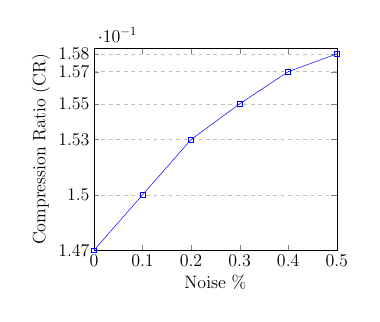
\begin{tikzpicture}[scale=0.45]
\begin{axis}[
    %title={Temperature dependence of CuSO$_4\cdot$5H$_2$O solubility},
    xlabel={Noise \%},
    ylabel={Compression Ratio (CR)},
    xmin=0, xmax=0.5, 
    ymin=0.1467, ymax=0.158, scaled y ticks={base 10:1},
    xtick={0,0.1,0.2,0.3,0.4,0.5},
    ytick={0.1467,0.1498,0.1529,0.1549,0.1567,0.1577},
     label style={font=\Large},
    tick label style={font=\Large},
    %legend pos=north west,
    ymajorgrids=true,
    grid style=dashed,
]
 
\addplot[
    color=blue,
    mark=square,
    ]
    coordinates {
    (0,0.1467)(0.1,0.1498)(0.2,0.1529)(0.3,0.1549)(0.4,0.1567)(0.5,0.1577)
    };
    %\legend{c}
\end{axis}
\end{tikzpicture}
\caption{When the noise increases, the compression ratio increases. Lower value of CR is preferred.} \label{fig:crnoise}
%\end{figure}
\label{fig:noise}
\end{minipage}
\hfill
\begin{minipage}[c]{0.4\linewidth}
%\begin{figure}
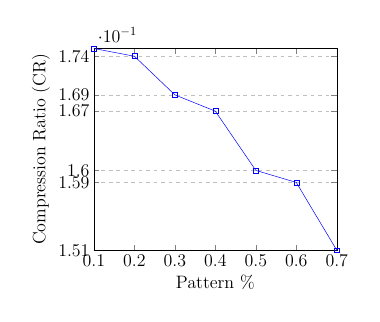
\begin{tikzpicture}[scale=0.45]
\begin{axis}[
    %title={Temperature dependence of CuSO$_4\cdot$5H$_2$O solubility},
    xlabel={Pattern \%},
    ylabel={Compression Ratio (CR)},
    xmin=0.1, xmax=0.7, 
    ymin=0.1510, ymax=0.1745, scaled y ticks={base 10:1},
    xtick={0.1,0.2,0.3,0.4,0.5,0.6,0.7},
    ytick={0.1736,0.1691,0.1672,0.1603,0.1589,0.1510},
    label style={font=\Large},
    tick label style={font=\Large},
    %legend pos=north west,
    ymajorgrids=true,
    grid style=dashed,
]
 
\addplot[
    color=blue,
    mark=square,
    ]
    coordinates {
    (0.1,0.1745)(0.2,0.1736)(0.3,0.1691)(0.4,0.1672)(0.5,0.1603)(0.6,0.1589)(0.7,0.1510)
    };
    %\legend{c}
\end{axis}
\end{tikzpicture}
\caption{When number of patterns increase, the compression ratio decreases. n=50, m=150, e=25} \label{fig:addpatterns}
%\end{figure}
\label{fig:pattern}
\end{minipage}%
\end{figure}  


\begin{figure}[h!]
\begin{minipage}[t]{0.22\textwidth}
\includegraphics[width=\linewidth,keepaspectratio=true]{images/random.pdf}
   \caption{For each model in Table \ref{tab:syn1000} we generated 100,000 random models with a random assignment of cuts for segments and local clusters. Red dots represents the optimal code length for each dataset found by our optimization algorithm.}
    \label{fig:random}
\end{minipage}
\hspace*{\fill}
\begin{minipage}[t]{0.23\textwidth}
\includegraphics[width=\linewidth,keepaspectratio=true]{images/ebola.pdf}
   \caption{Recorded weekly cases of Ebola infections for 15 counties in Liberia. Here, each county is a colored event sequence. The algorithm segments  the time on week 13 and the local clusters, presented in Table \ref{tab:ebola}, tell a story consistent with the analysis made by experts in the field of epidemiology. 
}
  \label{fig:ebola}
\end{minipage}
\end{figure}  

\subsection{Real Data}
\label{sec:realdata}
\subsubsection{Summarization of Ebola Virus Disease cases}
We analyze data from an agent-based model framework developed for forecasting the 2014-2015 Ebola epidemic in Liberia \cite{VENKATRAMANAN:2018}. We have the recorded weekly cases of Ebola infections for the 15 counties in Liberia. Figure \ref{fig:ebola} shows the cases and each county is a colored event sequence. The algorithm segments  the time on week 13 and the local clusters, presented in Table \ref{tab:ebola}, tell the following story consistent with the analysis made by experts in the field of epidemiology. For the first 13 weeks Grand Cape Mount is on it's own cluster with 203 cases. The second cluster groups Bomi and Gbarpolu with the highest counts with 79 and 28. cases. The rest of counties are clustered with 9 to 0 cases for the 13 weeks. The segmentation of week 13 is important because certain practices were enforced after that week. Traditional burial practices were observed among all communities which involves washing/touching/kissing the bodies during ceremony. The practices are confirmed to contribute to the spreading of Ebola Virus Disease (EVD). No effective safe burial protocol has been enforced till week 13. Also, no contact tracing cases were followed till week 13 and no Ebola Treatment Unit (ETU) were opened till week 13. 
 
From Table \ref{tab:ebola} it is easy to see that cases are high through the 20 weeks in Grand Cape Mount and Bomi. But Gbarpolu, from having a high number of cases from week 1 to 13, descends to a low level cluster 4 in week 14.
 
\begin{table}[!h]
\centering
    \caption{Summarization of Ebola virus disease confirmed cases in Liberia, 2015.}     
    \label{tab:ebola}
    \begin{small}
\begin{tabular}{p{0.35in}p{0.3in}p{2.3in}}
    \hline
    {\bfseries Segment} &{\bfseries Weeks} & {\bfseries  Clusters}   \\
    \hline
    1&1-13&  {\bfseries 1:} Grand Cape Mount    \\
    & & {\bfseries 2:}  Gbarpolu, Bomi   \\
    & & {\bfseries 3:} Bong, Montserrado, Lofa, Margibi, Grand Bassa, Grand Gedeh, Grand Kru, Maryland, Nimba, River Gee, Rivercess, Sinoe\\    \hline
     2&14-20 & {\bfseries 1:} Grand Cape Mount   \\
     & & {\bfseries 2:}  Bong, Bomi   \\
     & & {\bfseries 3:}  Margibi, Montserrado   \\
     & & {\bfseries 4:}  Gbarpolu, Lofa, Grand Bassa   \\
     & & {\bfseries 5:}  Nimba,Grand Gedeh, Grand Kru, Maryland, River Gee, Rivercess, Sinoe\\    \hline
    \end{tabular}
    \end{small} 
\end{table}

\subsubsection{Summarization of Global Landslides}
The Global Landslide Catalog (GLC) was developed with the goal of identifying rainfall-triggered landslide events around the world. The GLC considers all types of mass movements triggered by rainfall, which have been reported in the media, disaster databases, scientific reports, or other sources and has been compiled since 2007 at NASA Goddard Space Flight Center \cite{Kirschbaum:2010}. 
From the GLC, we analyze almost ten years (from 01/01/2007 to 10/25/2016) of reports of fatalities by landslides. 
%Figure \ref{fig:fatalities} shows the event sequences of fatalities by landslides for $m=102$ countries in $n=3586$ days; we can see how it's not trivial to define patterns and important segments in time from the plot. 
For this dataset the summarization outputs 9 segments and the corresponding local clusters are detailed in Table \ref{tab:landslide}.

%\begin{figure}[!tbh] 
 % \begin{center}
  %     \includegraphics[trim = 0in 1.7in 0in 1.8in, clip,scale=0.35]{images/landslide.pdf}
 % \end{center}
 %  \caption{Reports of landslides fatalities occurrences from 01/01/2007 to 10/25/2016 (3586 days), from the Global Landslide Catalog (GLC). Our model summarizes the dataset providing 9 %segments in time (represented in the Figure with different colors) and local clusters detailed in Table \ref{tab:landslide}.
%}
%  \label{fig:fatalities}
%\end{figure}


\begin{table}[!h]
\centering
    \caption{Summarization of Fatalities by landslides from the Global Landslide Catalog, from 01/01/2007 to 10/25/2016.}     
    \label{tab:landslide}
    \begin{small}
\begin{tabular}{p{0.35in}p{0.55in}p{0.6in}p{1.2in}}
    \hline
    {\bfseries Segment} &{\bfseries Begin Day} &{\bfseries Begin Date} & {\bfseries  Clusters}   \\
   &{\bfseries End Day} &{\bfseries End Date} &  \\
    \hline
    1&1 & 01/01/2007&{\bfseries 1:} All countries    \\
      &1237& 05/21/2010&   \\
    \hline
        2&1238 & 05/22/2010&{\bfseries 1:} China   \\
      &1313& 08/05/2010&  {\bfseries 2:} All other countries    \\
    \hline
        3&1314 & 08/06/2010&{\bfseries 1:} China   \\
      &1315& 08/07/2010&  {\bfseries 2:} India    \\
       && &  {\bfseries 3:} Pakistan    \\
       && &  {\bfseries 4:} All other countries     \\
    \hline
            4& 1316 & 08/08/2010&{\bfseries 1:} All countries   \\
      & 2800 & 08/31/2014&     \\
     \hline
      5& 2801 & 09/01/2014&{\bfseries 1:} India   \\
      & 2823 & 09/23/2014&  {\bfseries 2:} China, Pakistan  \\
      &  & &  {\bfseries 3:} All other countries  \\
     \hline
       6& 2824 & 09/24/2014&{\bfseries 1:} All countries   \\
      & 2972 & 02/19/2015&   \\
     \hline
        7& 2973 & 02/20/2015&{\bfseries 1:} All countries   \\
      & 2973 & 02/20/2015&   \\
      &  & &  \\
     \hline
        8& 2974 & 02/21/2015&{\bfseries 1:} All countries   \\
      & 3502 & 08/02/2016&   \\
     \hline
      9& 3503 & 08/03/2016&{\bfseries 1:} China   \\
      & 3586 & 10/25/2016& {\bfseries 2:} All other countries   \\
     \hline
    \end{tabular}
    \end{small} 
\end{table}

Segment 1 from 01/01/2007 to 05/21/2010 detects similar patterns for all countries. Segment 2 from 05/22/210 to 08/05/2010 detects, a high number of fatalities for China (2121), compared to other countries. It is interesting how segment 3, selects two days suggesting peaks in events and fatalities. During these 2 days, fatalities were only reported by China (1765), India (427) and Pakistan (58); there was one fatality reported from Trinidad and Tobago but this was clustered with the other countries with 0 reports. On 08/07/2010 in China, 1765 fatalities were reported by the cause of a landslide caused by heavy rainfall. On 08/06/2010 in India 427 fatalities were reported by the cause of a landslide caused by flash floods due to cloud burst in Leh in Ladakh region of North India. On 08/07/2010 in Pakistan, 58 fatalities were reported by the cause of a landslide caused by heavy rainfall that raised water levels in rivers. Segment 4, detects consistently high occurrences of landslides in all countries with the peak of landslide fatalities in 2013 to the event in Kedarnath, India which killed 5669 people. Segment 5 detects a similar pattern from segment 3 where India, China and Pakistan have high occurrences of landslides from 09/01/2014 to 09/23/2014. Segment 9 detects 50 fatalities in China from 08/03/2016 to 10/25/2016. This is an interesting global pattern corroborated by previous studies \cite{Kirschbaum:2010}, stating that landslide reports and landslides with fatalities peak in July through September, during the Northern Hemisphere summer, corresponding to the Southwest, South, and East Asian
monsoon seasons and the Northern Hemisphere tropical cyclone peaks. Segments 6 through 8 don't show high occurrences of landslides but Segment 7 selects one day in the dataset where there are no reports from any country in the world, 02/20/2015. 

\subsection{Results and Discussion}

For the synthetic dataset our model 1) effectively summarizes event sequences finding correct cuts and clusters in a dataset with 0.4\% of added noise. 2) The model efficiently performs summarization decreasing the compression ratio when the number of patterns increases. 3) By performing random cuts and clusters in a dataset the resulting global model cost is higher than our optimal summarization cost. For the real world dataset our model 1) find useful patterns, for example from the GLC dataset, the global pattern corroborated that landslide reports and landslides with fatalities peak in July through September corresponding to the Southwest, South, and East Asian
monsoon seasons \cite{Kirschbaum:2010}. 2) The summarization is easy to understand as we can see from Table \ref{tab:ebola} and Table \ref{tab:landslide}.





\section{Related Work}
Event summarization is closely related to sequential pattern and frequent episode mining. 
\subsection{Sequential pattern mining}
The sequential pattern mining problem was first introduced by Agrawal et al \cite{Agrawal:1995}, where Apriori based methods are used to mine frequent subsequences patterns from a sequence database. The main focus is on the patterns present on different transactions considering their sequential order. The output is frequent event subsequences with occurrence frequency bounded by a given threshold.  Alternatives to the method in \cite{Agrawal:1995} have been proposed and can be classified in Apriori-based 
\cite{Garofalakis:1999,Zaki:2001,Ayres:2002} 
%\cite{Srikant:1996,Garofalakis:1999,Zaki:2001,Ayres:2002} 
and pattern-growth based 
\cite{jianpei:2004,Pei:2007} 
%\cite{Han:2000,jianpei:2000,jianpei:2004,Pei:2007} 
algorithms. A limitation of these previous algorithms is that they don't provide a global description or 
%attempt to 
summarize redundant patterns. 
%Also, finding patterns is more complicated for sequences than for item sets.
\subsection{Frequent episode mining}
Frequent episode mining finds temporal patterns in event sequences. An episode is defined as a collection of events that occur relatively close to each other with respect to a timeline. In 
%\cite{Mannila1997,Achar2012,Achar:2013,Patnaik:2012} 
\cite{Mannila1997,Patnaik:2012} 
given a window size $w$ an episode containing an event pattern is frequent if it's frequency is bounded by a given threshold. As with the sequential pattern mining, frequent episode mining does not provide a global view of the event sequence. Also, parameters like the window size $w$ and thresholds have to be defined. 
\subsection{Frequent item set summarization}
To tackle the limitations of frequent item set mining, like redundancy and interpretability, frequent item set summarization has been proposed. The pattern profile method \cite{Yan:2005} aims to summarize the frequent patterns. K clusters contain the set of frequent patterns. Each cluster is described by a pattern profile. Based on the restoration error, a quality measure function determines the optimal value of parameter K. Also, the Markov Random Field method (MRF) \cite{Wang:2006}, for frequent item set summarization, models the items in the dataset as random variables. A MRF on these variables is constructed based on frequent itemsets and their occurrence statistics. We can see how these summarization methods focus on transaction type data and usually the time information is not considered.
\subsection{Event summarization}
Even summarization methods present summaries that consider the temporal dynamics of the events. Naturally temporal, events are generally stored as logs and overlooking the time dimension has severe implications in evaluating design decisions. Different methods of event summarization can be classified between two categories frequency change \cite{Kiernan:constructing,wang:algo} and temporal dynamics \cite{jiang:natural,Peng:2007,Schneider:2010,Tatti:2012}. Our model uses a frequency change approach providing a segmentation model. Each segment is described by a local model where the event types are grouped and clustered by frequency similarity. The temporal dynamics approach intents to reveal how the sequence changes over time. Our model does this through the temporal dynamics among the events in a segment and by selecting relevant segments with the minimum cost for description. %Because we want our algorithm to be parameter free, MDL \cite{Grunwald:2007} is at the core of our model by selecting the segments in the timeline and their local models that minimize the encoding length of the data without loosing accuracy in the description.
\subsection{Minimum Description Length}
The MDL approach is a generic technique that has been used in sequential pattern mining for problems like clustering \cite{slim:2012}, missing value estimation \cite{Vreeken:2008} and anomaly detection \cite{Vreeken2011,Chakrabarti:1998}. MDL has also been used for event summarization \cite{Kiernan:constructing,wang:algo,jiang:natural,Tatti:2012} but our work is the first in using MDL for generalization for any event summarization method describing bv event sequences to be extended to dv event sequences.
\subsection{Time series segmentation}
At a high level our model relates to the problem of time series segmentation 
\cite{Keogh:2001,Karras:2007,Guo:multi}. 
%\cite{Keogh:2001,Keogh93,Karras:2007,Guha:2001,terzi:2006,Liu:novel,Guo:multi}. 
The segmentation problem can be defined as the best representation given a time series $T$ using the parameter $k$ segments. 
%Also, it can be defined as the best representation given a time series $T$ such that the maximum error for any segment does not exceed some specified threshold. 
%In the same way 
Also, it can be defined as the best representation given a time series $T$ such that the combined error for all the segment does not exceed some specified threshold. This work is not parameter free, for example usually a threshold and the size of the time window needs to be defined.  While some work uses MDL to segment time series by providing a parameter-free approach \cite{xu:2013,Hu2015} we are focusing in event sequences and not time series. 
%Also, to solve the volume and dimensionality problem in time series, many research has proposed alternatives for a higher-level representation. For example, the Discrete Fourier Transform (DFT) \cite{agrawal:similarity}, Discrete Wavelet Transform (DWT) \cite{chan:dwt} and Singular Value Decomposition (SVD) \cite{korn:svd}. However, one drawback with respect to analyzing log data is that the dimensionality reduction based approach looks for global correlation and therefore are more suitable for finding similar images and shapes than data that have time component and local correlations.



\section{Conclusion and Future Work}

This paper presents a parameter-free global summarization that creates optimal global summaries of discrete event signals patterns. We use the MDL principle to detect regularities and compress data. We apply two dynamic programming algorithms to optimally and automatically segment the sequences in time and cluster events to discover similarities in polynomial time. We generalize the generative model used for binary values event sequences for discrete values event sequences. Experiments on synthetic and real datasets demonstrate that our summarization produces high-quality results with an automated global summary revealing regularities in the data. Future work includes temporal dynamic analysis for the model output; and to include spatio-temporal characteristics in the model.  



%\section*{Acknowledgment}

%The preferred spelling of the word ``acknowledgment'' in America is without 
%an ``e'' after the ``g''. Avoid the stilted expression ``one of us (R. B. 
%G.) thanks $\ldots$''. Instead, try ``R. B. G. thanks$\ldots$''. Put sponsor 
%acknowledgments in the unnumbered footnote on the first page.


\bibliographystyle{IEEEtran}
\bibliography{sample-bibliography}

\end{document}
